\chapter*{Appendix A: Kriging metamodel}

\subsubsection{Introduction}
The kriging metamodel technique has already been introduced in chapter \ref{ch:4} however; to complete the description of the method, the numerical procedure and some implementation examples are presented in this appendix.

The kriging method was invented to get prediction of missing geostatics data (\citet{krige1951statistical}). However, this methodology has been further generalized and applied extensively to build metamodels for a large variety of applications.
The method can treat highly non linear output of an experiment and can be used to either interpolate or extrapolate responses from a sample set.

In this discussion $\hat{f}(\boldsymbol{\chi})$ is a model for the true function $f(\boldsymbol{\chi})$ and $\hat{y}$ is the model prediction of the true response, $y = f(\boldsymbol{\chi})$, that is evaluated at the point $\boldsymbol{\chi}$. 

After the exploration of the design possibilities the database produced is usually organized in a set $(\mathbf{x_i}, y(\mathbf{x_i}))$  $i=1,...,n$ where
\begin{itemize}
	\item $\mathbf{x_i}$ is the $i-th$ vector element containing the $k$ input parameters for the $i-th$ experiment realization;
	\item $y_i$ is the scalar response of the experiment for the vector of inputs $\mathbf{x_i}$ \footnote{$y_i$ is always a scalar because even in case of multiple outputs for an experiment they are supposed to be uncorrelated. It means that if we had $p$ elements in each $\mathbf{y_i}$ we would have to build $p$ metamodels.};
	\item $\chi$ is the new input vector for which we seek the approximate output $\hat{y}=\hat{f}(\boldsymbol{\chi})$.
\end{itemize}

\subsubsection{Mathematical modelling}
We define with $n$ the number of points in the sample design set and with $k$ the number of inputs of the experiment; the $n \times k$ matrix containing all the inputs is indicated with $\mathbf{X}$ and the $n \times 1$ vector containing all the responses is indicated as $\mathbf{Y}$.

The kriging response for a new input point $\boldsymbol{\chi}$ is given by the linear \textit{predictor}:
\begin{equation}
\hat{y} = \hat{f}(\boldsymbol{\chi}) = \sum_{i=1}^{N} \lambda_i(\boldsymbol{\chi}) f(\mathbf{x_i}) =  \sum_{i=1}^{N} \lambda_i(\boldsymbol{\chi}) y_i,
\end{equation}

\noindent $\hat{y}$ is considered to be a new realization of the random Gaussian process that has generated the set of responses $\mathbf{Y}$.
The weights $\lambda_i$ are the solutions of a linear system obtained by minimizing the variance of the error between the predictor and the random process.
The best \textit{linear unbiased predictor} BLUP is obtained finding the weights $\lambda_i$ that minimize:

\begin{equation}
MSE[\hat{y}(\chi)] =  E \left[\left( \hat{f}(\boldsymbol{\chi})  -f(\boldsymbol{\chi}) \right)^2\right] = E \left[\left(   \boldsymbol{\lambda}^T(\boldsymbol{\chi})\mathbf{Y} -y(\chi)\right)^2\right],
\label{eq:var_err}
\end{equation}

\noindent under the unbiasedness condition:

\begin{equation}
E \left[ \hat{f}(\chi)  -f(\chi)\right] =  E \left[ \boldsymbol{\lambda}^T(\boldsymbol{\chi})\mathbf{Y} -\mathbf{y}(\boldsymbol{\chi})  \right] = 0.
\label{eq:unb_cond}
\end{equation}
This relation means that the predictor and the Gaussian process have the same mean value for every new point $\boldsymbol{\chi}$. The equation \eqref{eq:unb_cond} is further developed yielding:
\begin{equation}
E \left[ \hat{f}(\chi)  -f(\chi)\right] = \boldsymbol{\lambda}^T \boldsymbol{\chi} E \left[ f(\mathbf{X})  \right] - E \left[ f(\boldsymbol{\chi})  \right] = \sum_{i=1}^{n} \lambda_i(\boldsymbol{\chi}) \mu(\mathbf{x_i}) - \mu(\boldsymbol{\chi}) = 0,
\label{eq:unb_cond2}
\end{equation}
where $\mu(\boldsymbol{\chi})$ is the mean value of the true function at the point $\boldsymbol{\chi}$; instead $\mu(\mathbf{x_i})$ is the mean of all the realizations collected for the database.

Different types of kriging approximation exist accordingly to how $\mu(\boldsymbol{\chi})$ is evaluated:
\begin{itemize}
	\item \textbf{simple kriging} assume that the trend has null value: $\mu(\boldsymbol{\chi}) = 0$;
	\item \textbf{ordinary kriging} assume that the trend is an unknown constant: $\mu(\boldsymbol{\chi}) = \mu$;
	\item \textbf{universal kriging} assumes that the trend is the solution of a generalized \textit{least squares model} in which it is possible to decide the order ($n_{\beta}$)\footnote{This means that, for example, taking $n_{\beta}= 2$ the least squared model is quadratic.} of the chosen base: $\mu(\boldsymbol{\chi}) = \mathbf{g}^T(\boldsymbol{\chi}) \boldsymbol{\beta}$, where $\mathbf{g}(\boldsymbol{\chi})$ is the base evaluation at the point $\boldsymbol{\chi}$ and the vector $\boldsymbol{\beta}$ contains the $n_{\beta}$ coefficients of the model.
\end{itemize}

The unbiased condition \eqref{eq:unb_cond2} can be so rewritten, without loss of generality:
\begin{eqnarray}
 \boldsymbol{ \lambda}^T (\boldsymbol{\chi}) \mathbf{G}(\mathbf{X}) \boldsymbol{\beta} - \mathbf{g}^T(\boldsymbol{\chi}) \boldsymbol{\beta} = 0 \Longrightarrow \boldsymbol{\lambda}^T(\boldsymbol{\chi}) \mathbf{G}(\mathbf{X}) = \mathbf{g}^T(\boldsymbol{\chi}),
\end{eqnarray}
where $\mathbf{G}(\mathbf{X})$ is the $n \times n_{\beta}$ matrix containing the evaluation of the least squared basis functions at all points in $\mathbf{X}$.

Also the relation \eqref{eq:var_err} can be manipulated:
\begin{eqnarray}
E \left[\left( \hat{f}(\boldsymbol{\chi})  -f(\boldsymbol{\chi}) \right)^2\right] &=& var(  \hat{f}(\boldsymbol{\chi})  -f(\boldsymbol{\chi}) ) \nonumber \\
&=& var(\hat{f}(\boldsymbol{\chi}))  +var(f(\boldsymbol{\chi})) -2 \; cov( \hat{f}(\boldsymbol{\chi}),f(\boldsymbol{\chi})) \nonumber \\
&=& var( \sum_{i=1}^{n}\lambda_i(\boldsymbol{\chi}) f(\mathbf{x_i}) )  +var(f(\boldsymbol{\chi})) -2 \; cov( \sum_{i=1}^{n}\lambda_i(\boldsymbol{\chi}) f(\mathbf{x_i}),f(\boldsymbol{\chi})) \nonumber \\
&=&  \sum_{i=1}^{n} \sum_{j=1}^{n} \lambda_i(\boldsymbol{\chi})\lambda_j(\boldsymbol{\chi}) \; cov(f(\mathbf{x_i}),   f(\mathbf{x_j})) +var(f(\boldsymbol{\chi})) \nonumber \\
&& \qquad \qquad \qquad -2 \;  \sum_{i=1}^{n}\lambda_i(\boldsymbol{\chi}) \; cov(f(\mathbf{x_i}),f(\boldsymbol{\chi})) \nonumber \\
&=& \sum_{i=1}^{n} \sum_{j=1}^{n} \lambda_i(\boldsymbol{\chi})\lambda_j(\boldsymbol{\chi}) \; cov(\mathbf{x_i}, \mathbf{x_j}) +var(f(\boldsymbol{\chi})) \nonumber \\
&& \qquad \qquad \qquad -2 \;  \sum_{i=1}^{n}\lambda_i(\boldsymbol{\chi}) \; cov(\mathbf{x_i},\boldsymbol{\chi}),
\label{eq:BLURP}
\end{eqnarray}
where $\mathbf{c} = cov(\mathbf{X},\boldsymbol{\chi})$ is the vector containing the estimated covariance between each point in the input set $\mathbf{X}$ and the point $\boldsymbol{\chi}$ for which we search the estimator. Similarly, $\mathbf{C}_{ij} =  cov(\mathbf{x_i}, \mathbf{x_j})$ represents the elements in the $n \times n$ matrix containing the correlation estimates between each point in $\mathbf{X}$. Possible estimations for the two covariance matrixies are listed in the next section.

The derivative of the relation \eqref{eq:BLURP} with respect to $\boldsymbol{ \lambda}$ is posed equal to zero in order to minimize the kriging error, yielding the final relation:
\begin{equation}
\boldsymbol{\lambda}^T(\boldsymbol{\chi}) \mathbf{C} = \mathbf{c}.
\end{equation}

Introducing the Lagrangian multiplier $\phi$ for the unbiased constraint it is possible to build the partitioned matrix for the kriging metamodel:
\begin{equation}
\left(
\begin{array}{c c}
\mathbf{0} & \mathbf{G}^T \\
\mathbf{G} & \mathbf{C}
\end{array}
\right)  \left( 
\begin{array}{c}
\boldsymbol{\phi} \\
\boldsymbol{\lambda}
\end{array}
\right) = \left( 
\begin{array}{c}
\mathbf{g} \\
\mathbf{c}
\end{array}
\right).
\end{equation}

\noindent Then, by inverting the partitioned matrix the kriging predictor can be written as:
\begin{equation}
\hat{y}(\boldsymbol{\chi}) = \mathbf{g}^T(\boldsymbol{\chi}) \boldsymbol{\beta} + \mathbf{c}^T(\boldsymbol{\chi}) \mathbf{R}^{-1} \left( \mathbf{Y} - \mathbf{G}\boldsymbol{\beta} \right).
\end{equation}

The first term $\mathbf{g}(\boldsymbol{\chi})^T \boldsymbol{\beta}$ is usually called \textit{trend function} and the second term is the \textit{Gaussian error model}. As a matter of fact, $\left( \mathbf{Y} - \mathbf{G}\boldsymbol{\beta} \right)$ is the known vector of differences between the true outputs and the trend function at all the points $\mathbf{X}$ in the database.

One of the kriging metamodel benefits is that the model is exact at the data points. However, if it is known that the experimental realization used in the database presents some reliability issue and/or have noise\footnote{common in experimental data.}, there is a technique that permits to take into account these effect.
Adding a \textit{nugget} ($\eta$) to all entries on the covariance matrix $\mathbf{C}^* = \mathbf{C} + \eta \mathbf{I}$ the metamodel is no more exact at the data points. The same technique is used to increase the conditioning number of the portioned system when dealing with numerical problems.

\subsubsection{Covariance matrix choice}
\label{sec:cov}

In order to give some indication on the choice of the proper covariance function let us first introduce the \textit{semivariogram} concept.
The semivariogram $\gamma$ between two generics points, in the design space  $\mathbf{x_1}, \mathbf{x_2}$, is defined as:
\begin{eqnarray}
\gamma(\mathbf{x_1}, \mathbf{x_1}) &=& \dfrac{1}{2} E \left[  (f(\mathbf{x_1}) -\mu(\mathbf{x_1}) -f(\mathbf{x_2}) +\mu(\mathbf{x_2}))^2 \right] \label{eq_semvar1}\\
&=& \dfrac{1}{2} var(f(\mathbf{x_1}) -f(\mathbf{x_2}) ) \nonumber \\
&=& \dfrac{1}{2} var(f(\mathbf{x_1}))  +\dfrac{1}{2} var(f(\mathbf{x_2})) -cov(\mathbf{x_1}, \mathbf{x_2}) \label{eq_semvar2}
\end{eqnarray}

The semivariogram for each datapoint in the database can be directly computed from the equation \eqref{eq_semvar1} and afterwards the relation \eqref{eq_semvar2} can be used to fit the semivariogram data with the covariance function.

Lets us clarify the last statements with an example. We chose to replicate the example present in \citet{cavazzuti2012optimization} in which the author proposes an experiment that depends on two variables $x_1$ and $x_2$ and $10$ realizations. The experiment database is shown in figure \ref{fig:doedata}.

\begin{figure}[t]
	\centering
	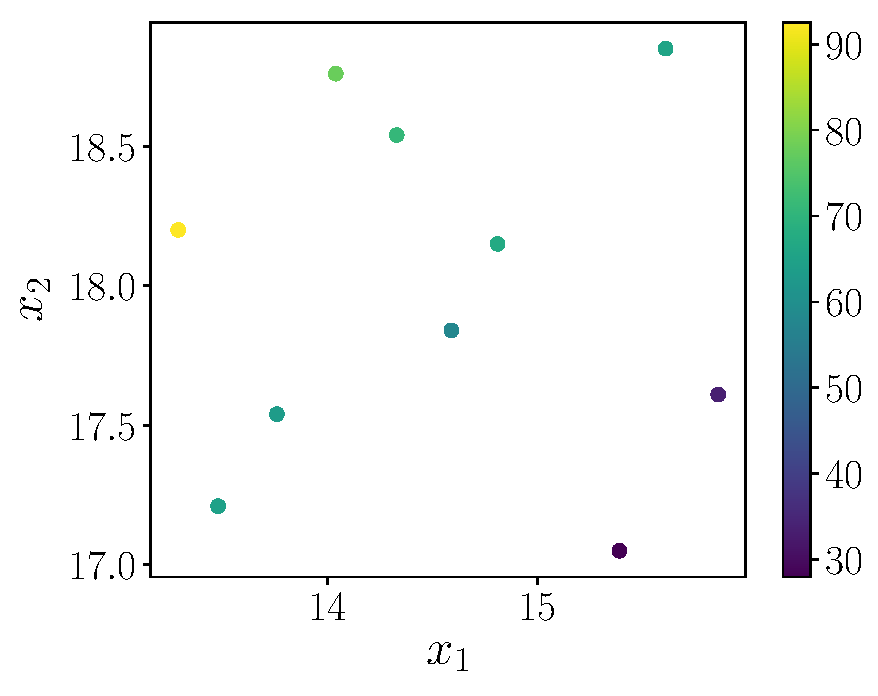
\includegraphics[width=0.5\linewidth]{appendix_a/DOE_data}
	\caption{Experiment data points for the $10$ realizations available. The color map represent the output realizations  $\mathbf{Y}$ of the experiment $f(\mathbf{X})$.}
	\label{fig:doedata}
\end{figure}

The semivariogram functions, as a function of the Eucledian distance between the two points $h_{ij} = |\mathbf{x}_i - \mathbf{x}_j|$, has been computed using equation \eqref{eq_semvar1} and is represented in figure \ref{fig:semivariogram} on the left. The points in the semivariogram are then averaged over a distance step whose width is equal to $0.25$ and the points are shown on the right of figure \ref{fig:semivariogram}.
The correlation function should be chosen to be the best fit for the averaged semivariogram. This means that in theory, depending on the dataset, one could formulate a personalized covariance model.

\begin{figure}[ht]
	\centering
	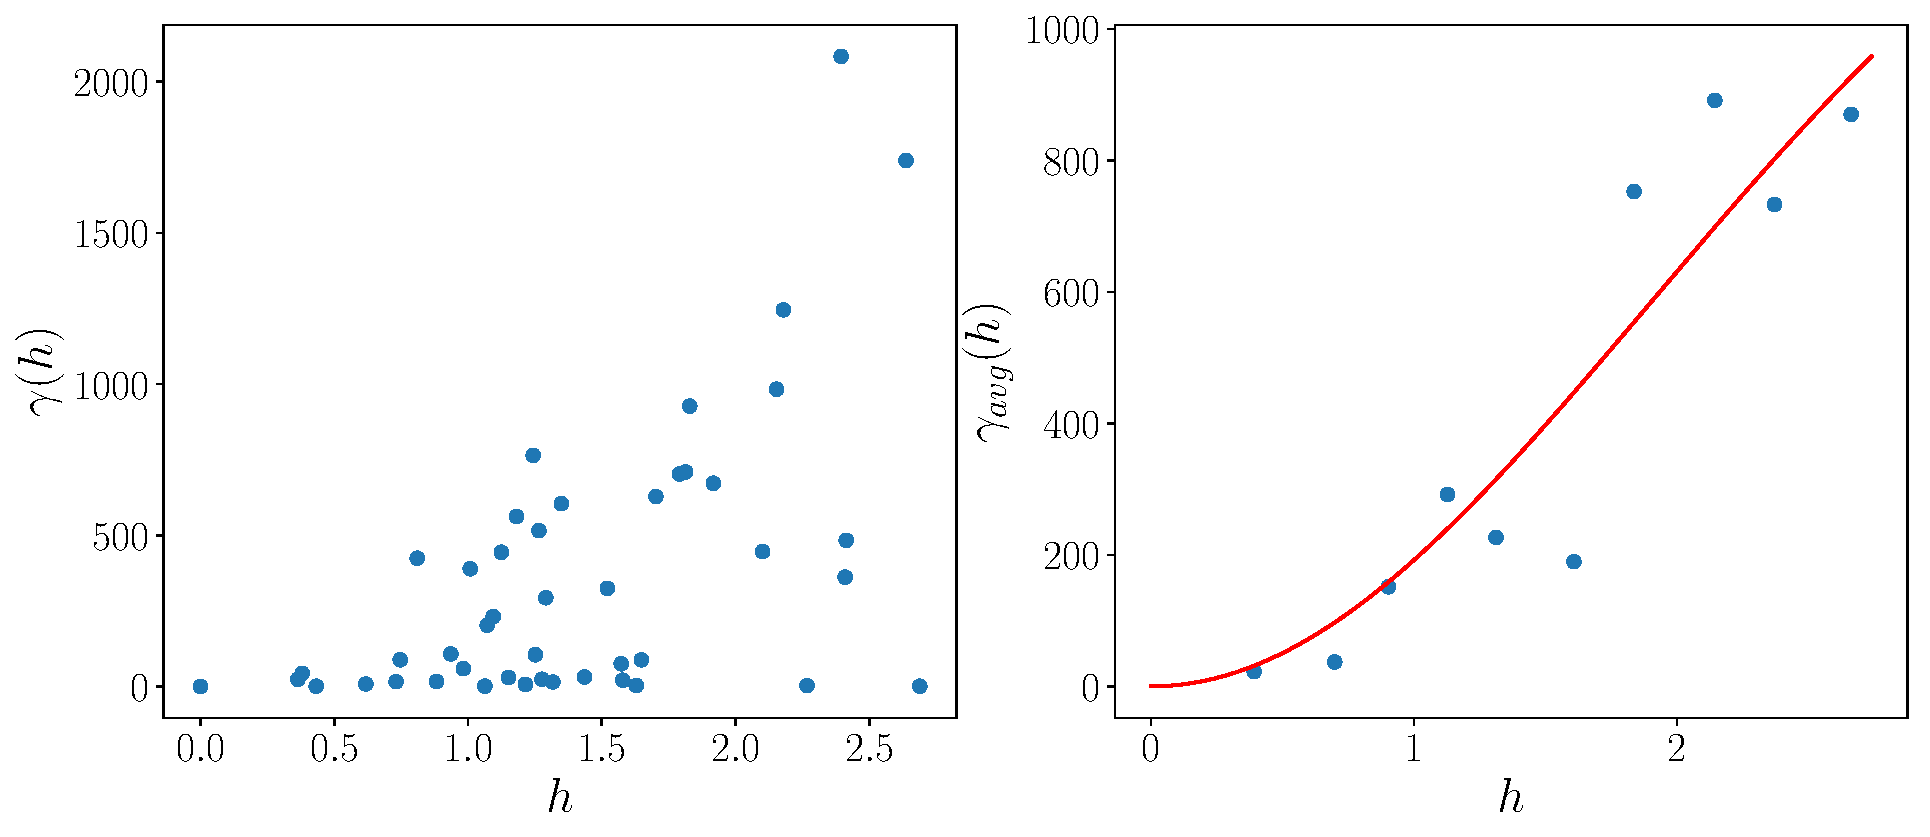
\includegraphics[width=0.9\linewidth]{appendix_a/sem}
	\caption{Left: Semivariogram versus the Euclidean distance computed for each data point against the other.  Right: The blue dots represents the same semivarigram on the left but averaged over a step distance equal to $0.25$. The red line corresponds to the semivariogram computed using relation \eqref{eq_semvar2} with the covariance model \textit{power exponential} with parameters $\nu=2$, $\theta=1.895$ and $\sigma=38.44$.}
	\label{fig:semivariogram}
\end{figure}

What is done in practice is that some parametric families of correlation functions have been proposed in the literature; for example the \textit{power exponential} correlation function reads:
\begin{equation}
c(\mathbf{x}_{i} , \mathbf{x}_{j})  = \sigma^2 \textrm{exp}\left( -\sum_{j=1}^{k} \theta_k {|{x}_{i,k} - {x}_{j,k} |}^\nu \right).
\end{equation}

The kriging predictor surfaces can show different behaviors for different selections of the above three parameters ($\sigma$, $\nu$ and $\boldsymbol{\theta}$) and their setting is thus crucial.
The coefficient $\sigma$ is an amplitude parameter for the correlation function. It determines variations of the function $\hat{f}$ from its mean. Small values of $\sigma$ characterize functions that stay close to their mean value, larger values allow more variations. It basically controls the gradient steepness around the data points. The exponent $\nu$ of the model has similar effects.
The vector $\bs{\theta}=(\theta_{x_1}, \theta_{x_2})$ is a length scale parameter for the distance $|\mathbf{x_i} - \mathbf{x_j}|$; describes how smooth a function is. Small length scale values mean that function values can change quickly generating narrow bumps near the data points. Large values characterize functions that change only slowly but it will make the surface explode outside the convex hull described by the data points. It is possible to specify different length scales in different directions, in this manner the metamodel can include anisotropic effect for each variable of the experiment.
This model has been fitted in the previous semivariogram choosing $\nu=2$, $\theta=1.895$ and $\sigma=38.44$ and it is depicted in the right figure \ref{fig:semivariogram} using a red line. Is possible to see that this model fits well the data points for this experiment.

Another popular model for the covariance function is the \textit{Mat\'ern model}\footnote{the one used in chapter \ref{ch:4}.} that reads:
\begin{equation}
c(\mathbf{x}_{i} , \mathbf{x}_{j}) = \sigma^2 \dfrac{2^{1- \nu}}{\Gamma(\nu)} \ \sum_{j=1}^{k} \left[ \left( \dfrac{\sqrt{2} \nu |{x}_{i,k} - {x}_{j,k} |}{\theta_k} \right)^{\nu} \ \mathcal{K}_{\nu}\left( \dfrac{\sqrt{2} \nu |{x}_{i,k} - {x}_{j,k} |}{\theta_k} \right) \right],
\label{eq:matern2}
\end{equation}
where $\mathcal{K}_{\nu}(.)$ is a modified Bessel function and $\Gamma(.)$ is the gamma function.
The parameters that can be used to tune the metamodel are the amplitude parameter $\sigma$, the exponent $\nu$ and the scale vector $\bs{\theta}$ with the same meaning as in the previous correlation function.

To summarize, when choosing the correlation it should be kept in mind:
\begin{itemize}
	\item to well approximate the trend of the averaged semivariogram,
	\item the scale parameter $\boldsymbol{\theta}$ highly changes the presence of spurious minima and maxima in the metamodel. The others parameters $\nu$, $\sigma$ and $\eta$ control the gradient and the exactness of the model around the data points.
\end{itemize}

Some examples of the response surface built with the above parameters are presented in the next section, along with the actual implementation.

\subsubsection{Implementation example}
An example of the implementation of kriging algorithm is presented in the following. To build the model we use the open source library openTURNS (\citet{openturns}) using its Python application programming interface\footnote{although the crunching number computation is performed under the hood with C++.}. This interface has been chosen because it is very expressive even to non programmers. 
The code is shown in the listing below where each line is commented and is self explanatory. From line 1 through 22 the experiment database is created, in line 24 the trend function model is set constant but line 26 and 28 show how to set linear and quadratic least square trends. The covariance model is set in line 31, and from line 35 to 42 the algorithm metamodel tree is built and executed. At the end it is possible to get a callable function on the desired new point, line 44-47.

%\begin{minted}[frame=lines, linenos=true]{c++}
%#include <iostream>
%int main() {
%	std::cout << "Hello "
%	<< "world"
%	<< std::endl;
%}
%\end{minted}


%\begin{listing}[ht]
\begin{minted}[frame=lines, linenos=true]{python}
	import numpy as np # import the generic vector library
	import openturns as ot # import the openTURNS library
	
	# define the k input varibles as a n dimensional array
	x1 = np.array([14.04, 14.33, 15.39, 13.76, 14.59,
				   13.48, 15.86, 15.61, 13.29, 14.81])
	x2 = np.array([18.76, 18.54, 17.05, 17.54, 17.84,
	               17.21, 17.61, 18.85, 18.20, 18.15])
	
	# transform the inputs as a n by k array
	x = np.column_stack((x1, x2))
	
	# define the outputs as  a n by 1 array
	y = np.array([[10],[2 ],[4],[-2],[9],[3] ,[0], [-1]])
	
	# tranform the array in OT samples
	X = ot.Sample(x)
	Y = ot.Sample(y)
	
	# explicit define the number of input i.e the k number
	dimension = len(x[0])
	
	# define the constant trend function
	basis = ot.ConstantBasisFactory(dimension).build()
	# or the linear trend
	# basis = ot.LinearBasisFactory(dimension).build()
	# or the quadratic trend
	# basis = ot.QuadraticBasisFactory(dimension).build()
	
	# select the covariance model squared exponential (sigma, theta)
	covarianceModel = ot.SquaredExponential([38.44], [1.895])
	# or define the Matern model
	# covarianceModel = ot.MaternModel()
	
	algo = ot.krigingAlgorithm(X, Y, covarianceModel, basis) # build the metamodel
	
	# eta = 0.2
	# algo.setNoise([eta]*len(y)) # set the optional nugget
	
	algo.run() # run the metamodel tree computation
	result = algo.getResult() # return a container for the results
	metamodel = result.getMetaModel() # get a callable function
	
	# set the new point to compute
	chi = np.array([13, 17])
	# get the metamodel prediction for the point chi
	y_chi = np.array(metamodel(chi))
\end{minted}
%\caption{Example of kriging metamodel implementation using openTURNS library.}
%\label{code}
%\end{listing}

\newpage

It is possible to pass directly a vector of new points to the function \textit{metamodel} in line 44. Figures \ref{fig:kriging_openturns}, \ref{fig:kriging_openturns2} and \ref{fig:kriging_openturns3} show some metamodel surfaces with different parameters setup.

\begin{figure}[t!]
\centering
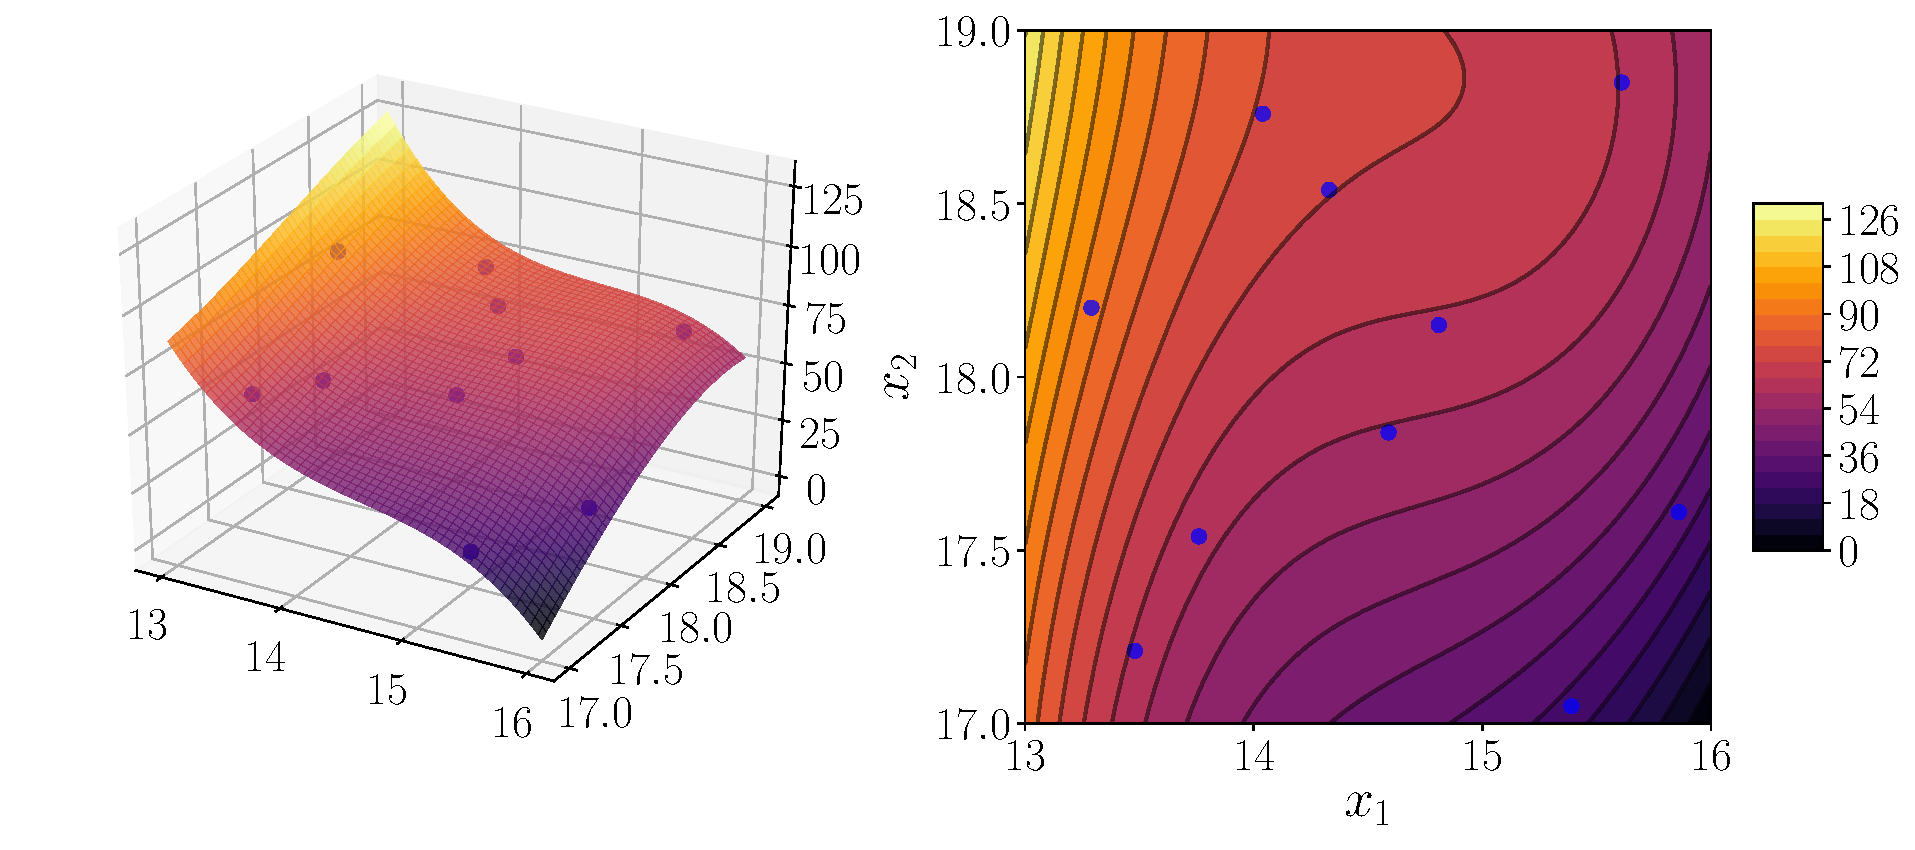
\includegraphics[width=0.9\linewidth]{appendix_a/kriging_openturns}
\caption{kriging metamodel surface for using a constant trend function and the \textit{power exponential} covariance model with parameters $\nu=2$, $\theta=1.895$ and $\sigma=38.44$.}
\label{fig:kriging_openturns}
\end{figure}

It is possible to see that changing the parameters of the kriging metamodel the shape of the response function can change, and some very bad choice of the parameters can lead to very exotic shapes, like in figure \ref{fig:kriging_openturns3}. In any case it is possible to test the robustness of a certain setup using an error estimate like the one proposed in chapter \ref{ch:4}. In practical applications the choice of the optimal parameters is usually left to the experience of the user.

\begin{figure}[h]
	\centering
	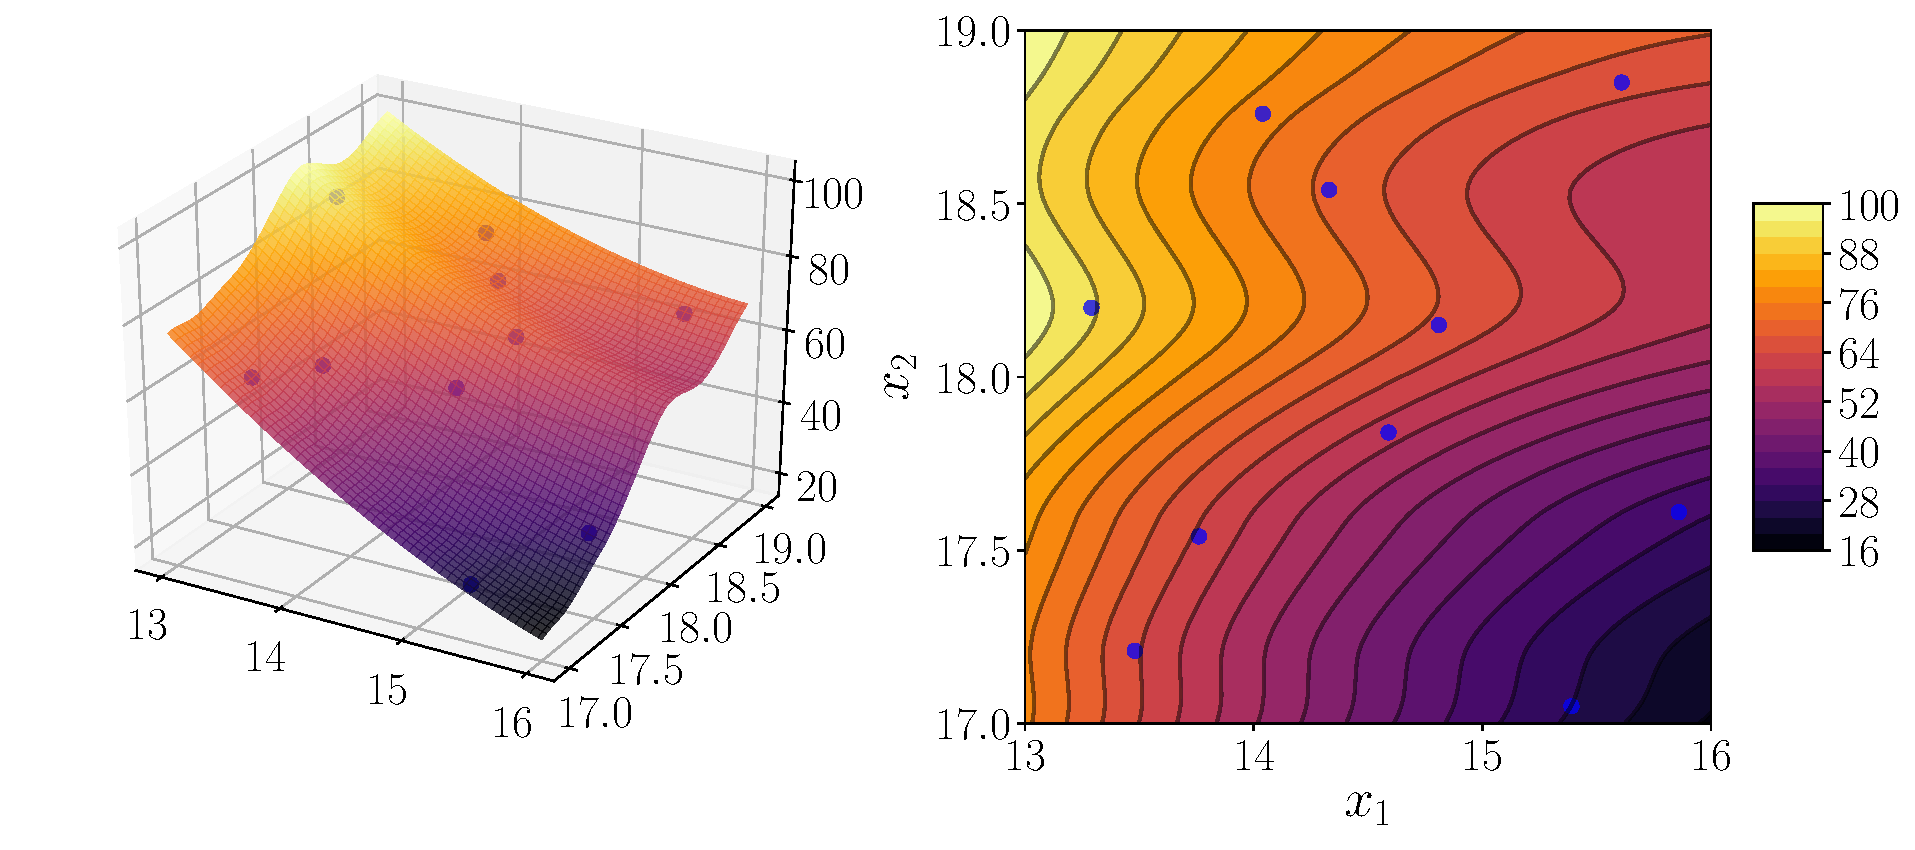
\includegraphics[width=0.9\linewidth]{appendix_a/kriging_openturns2}
	\caption{kriging metamodel surface for using a quadratic trend function and the \textit{Matern} covariance model with parameters $\nu=1.5$, $\theta=10$ and $\sigma=1$.}
	\label{fig:kriging_openturns2}
\end{figure}

\begin{figure}[h]
	\centering
	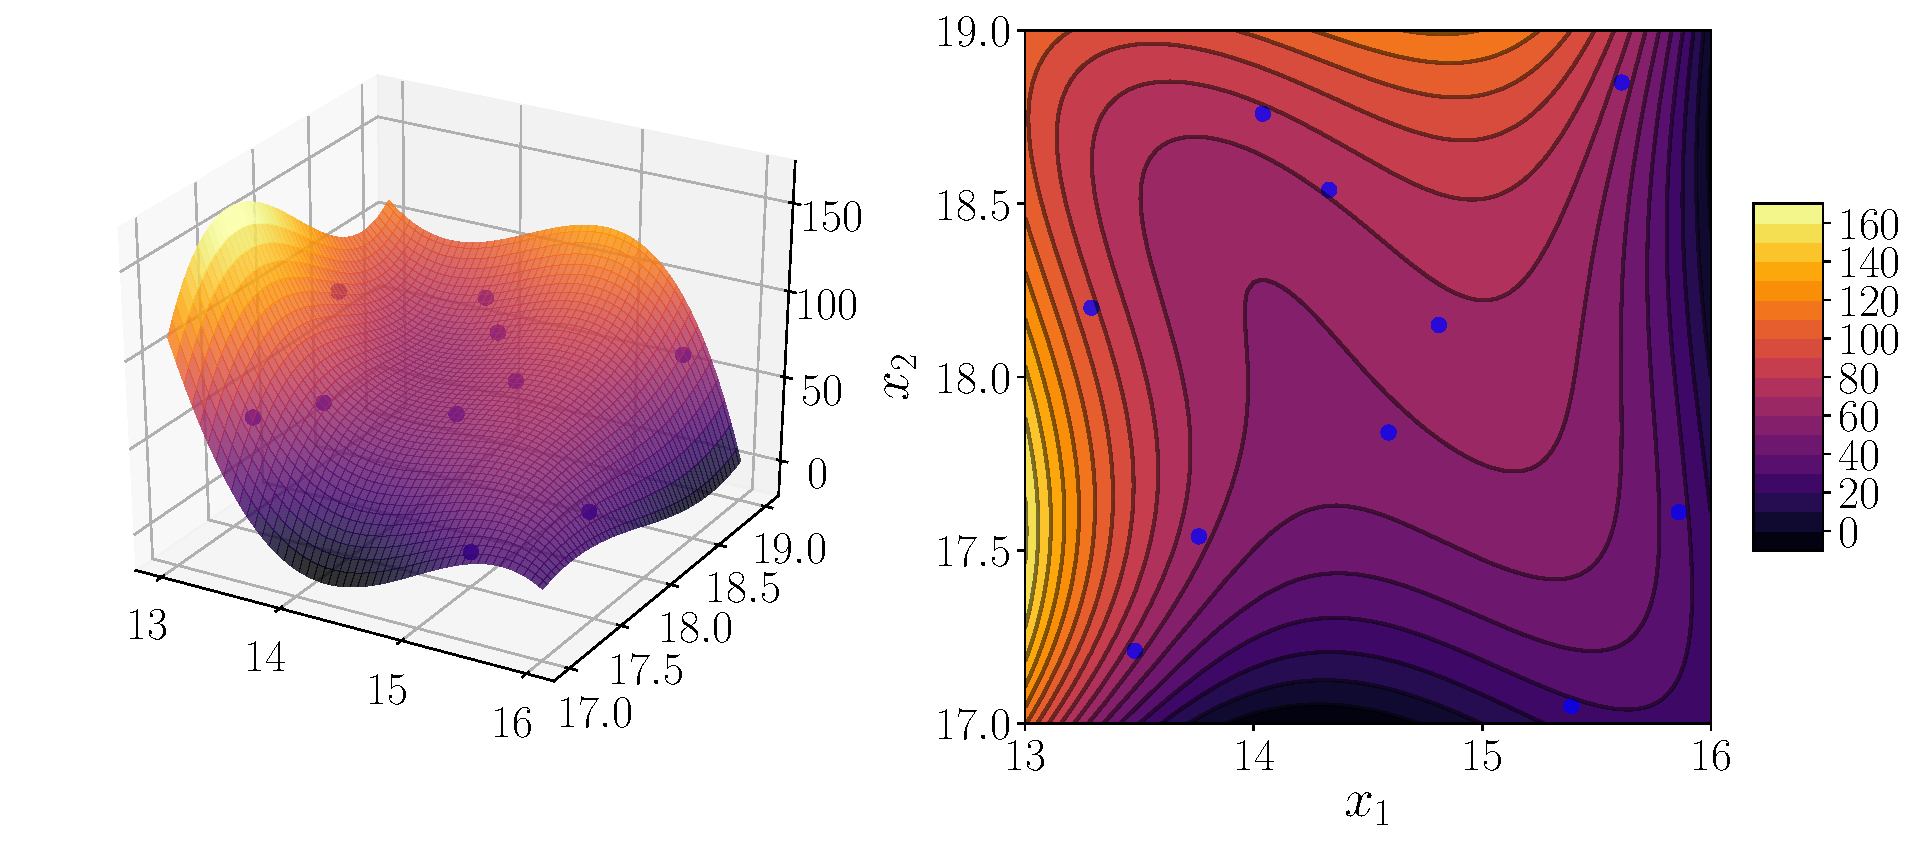
\includegraphics[width=0.9\linewidth]{appendix_a/kriging_openturns3}
	\caption{kriging metamodel surface for using a linear trend function and the \textit{power exponential} covariance model with parameters $\nu=2$, $\theta=0.8$ and $\sigma=10$.}
	\label{fig:kriging_openturns3}
\end{figure}


\subsubsection{Final remarks}
Further detail on theoretical and computational aspects can be found in \citet{cavazzuti2012optimization}, \citet{dakota}, \citet{sacks1989design} and \citet{openturns}.
The above code snippet is public, in the GitHub repository of the author can be found at the address: \url{https://github.com/appanacca/kriging_book.git}.
The OpenTRUNS library implementation is available at the previous repository link. In addition an equivalent ordinary kriging implementation, starting from scratch, can be downloaded.
More generally whenever a reduced order model has to be built with a not extremely large amount of data the Kriging metamodelling should be a solution to investigate seriously.
